% ============================================================================
% Chapitre 3 — Réalisation et implémentation
% ============================================================================
\chapter{Réalisation et implémentation}

Ce chapitre détaille la réalisation technique du projet~: environnement, \textit{stack}, constitution du dataset, pipeline \ac{RAG}, modules métier, \textit{backend} FastAPI et interface Next.js. Il se conclut par la structure du dépôt et les règles de développement adoptées.

\section{Environnement}

L'environnement de développement est résumé dans le tableau~\ref{tab:env}. Aucun service cloud payant n'est requis pour exécuter le système en local --- seule l'\ac{API} OpenAI implique une consommation à l'usage.

\begin{table}[H]
\centering
\caption{Environnement de développement.}
\label{tab:env}
\begin{tabularx}{\textwidth}{@{}l X@{}}
\toprule
\textbf{Élément} & \textbf{Valeur} \\
\midrule
Système d'exploitation        & Linux (Ubuntu) \\
Langage \textit{backend}      & Python 3.11+ \\
Langage \textit{frontend}     & TypeScript 5 \\
\ac{API} \ac{LLM}             & OpenAI (clé personnelle en \code{.env}) \\
IDE                           & Visual Studio Code \\
Gestion de version            & Git + GitHub \\
Environnement virtuel         & \code{venv} Python \\
Gestionnaire de paquets front & \code{npm} \\
\bottomrule
\end{tabularx}
\end{table}

\section{Stack technique}

Le choix des briques techniques a privilégié des composants matures, libres lorsque possible, et avec une empreinte locale raisonnable. Le tableau~\ref{tab:stack} en fournit la justification synthétique.

\begin{table}[H]
\centering
\caption{Stack technique et justifications.}
\label{tab:stack}
\small
\begin{tabularx}{\textwidth}{@{}l l X@{}}
\toprule
\textbf{Composant} & \textbf{Techno} & \textbf{Justification} \\
\midrule
Backend        & Python 3.11+                & écosystème \ac{NLP}/IA mature \\
Serveur \ac{API} & FastAPI + Uvicorn        & asynchrone, \ac{SSE} natif, Swagger auto-généré \\
\ac{LLM}       & OpenAI GPT-3.5-turbo       & qualité français correcte, température configurable \\
Embeddings     & \texttt{MiniLM-L12-v2}      & local, gratuit, multilingue (384 dim.) \\
Base vectorielle & ChromaDB                 & léger, persistant (SQLite), parfait pour la taille du dataset \\
Pipeline RAG   & LangChain                   & orchestration, \textit{chunking}, \textit{prompt templates} \\
Frontend       & Next.js 16 + React 19       & App Router, \textit{streaming} natif \\
Styling        & Tailwind CSS 4 + Radix UI   & \textit{utility-first}, composants accessibles \\
Animations     & Framer Motion               & fond animé, transitions fluides \\
Onboarding     & React Joyride               & tour interactif pour nouveaux utilisateurs \\
Configuration  & \code{python-dotenv}        & variables d'environnement \\
Tests          & \code{pytest}               & tests unitaires \\
\bottomrule
\end{tabularx}
\end{table}

\section{Constitution du dataset}

Le dataset a été construit entièrement \textbf{à la main}, sans \textit{scraping} automatisé, afin de garantir la qualité et la pertinence des données. Le volume total est d'environ 504~KB de données structurées et non structurées (figure~\ref{tab:dataset}). La couverture sectorielle comprend 28 domaines (fintech, \ac{SaaS}, e-commerce, \textit{healthtech}, \textit{edtech}, \textit{agritech}, etc.). La couverture géographique est centrée sur le Maroc, étendue à la France, à l'Afrique francophone et à la région \ac{MENA}.

La liste des 18 \ac{KPI} couverts est la suivante~:

\begin{itemize}
  \item \textit{Revenue}~: \ac{MRR}, \ac{ARR}, \textit{MRR Growth Rate}~;
  \item \textit{Unit economics}~: \ac{CAC}, \ac{LTV}, ratio LTV/CAC, \textit{CAC payback period}, \textit{gross margin}~;
  \item \textit{Opérationnel}~: \textit{burn rate}, \textit{runway}, \textit{churn rate}, \textit{net revenue retention}~;
  \item \textit{Marketplace}~: \ac{GMV}, \textit{take rate}~;
  \item \textit{Fintech}~: \ac{TPV}~;
  \item \textit{Engagement}~: \ac{DAU}/\ac{MAU}~;
  \item \textit{Satisfaction}~: \ac{NPS}.
\end{itemize}

La structure détaillée des fichiers \ac{JSON} est disponible en annexe~\ref{ann:dataset}.

\section{Pipeline RAG}

\subsection{Configuration centralisée}

Le module \code{backend/app/config.py} centralise les paramètres. Il charge le fichier \code{.env} depuis la racine du dépôt et expose~:

\begin{itemize}
  \item \code{OPENAI\_API\_KEY}, \code{LLM\_MODEL} (par défaut \code{gpt-3.5-turbo}), \code{EMBEDDING\_MODEL}~;
  \item \code{CHROMA\_PERSIST\_DIR} (par défaut \code{./chroma\_db})~;
  \item \code{CHUNK\_SIZE} / \code{CHUNK\_OVERLAP} (500 / 50)~;
  \item \code{TOP\_K} = 5~;
  \item \code{DATASET\_DIR} (par défaut \code{./dataset}).
\end{itemize}

\subsection{Chargement des données}

Le module \code{data\_loader.py} fournit une interface unifiée pour lire et valider les sources. Il expose six \textit{loaders} (\code{load\_investors()}, \code{load\_grants()}, \code{load\_metrics()}, \code{load\_faq()}, \code{load\_fundraising\_guides()}, \code{load\_regulations()}) et un agrégateur \code{load\_all()}. Chaque \textit{loader} gère ses erreurs sans lever d'exception fatale~: si un fichier est manquant, l'erreur est \textit{logguée} et un conteneur vide est retourné~; si un enregistrement est incomplet, un \textit{warning} est émis et l'enregistrement est écarté.

\subsection{Ingestion et chunking}

Le module \code{ingest.py} transforme chaque source en objets \code{Document}, attache les métadonnées appropriées, puis applique un \code{RecursiveCharacterTextSplitter}. Les six types traités sont~: \ac{FAQ} (question + réponse combinées), guides de \textit{fundraising}, régulations, investisseurs, subventions et métriques. Pour les investisseurs, par exemple, chaque profil est aplati en un paragraphe textuel riche (nom, type, secteurs, tickets, géographie, portefeuille) avant \textit{chunking}.

\subsection{Modèle d'embedding}

Le modèle retenu, \texttt{paraphrase-multilingual-MiniLM-L12-v2}, offre un compromis favorable~: 384 dimensions (stockage compact), support natif de 50 langues dont le français, taille du modèle de l'ordre de 130~MB, exécution sur \ac{CPU} sans \ac{GPU}. Aucun appel \ac{API} n'est requis pour la vectorisation, ce qui isole cette étape des pannes éventuelles d'un fournisseur externe.

\subsection{Base vectorielle et recherche}

Le module \code{vectorstore.py} expose deux fonctions~: \code{build\_vectorstore()} (reconstruction complète) et \code{get\_vectorstore()} (chargement rapide depuis le disque). La collection est nommée \code{tamwil\_knowledge\_base} et est persistée sur disque via le \textit{backend} SQLite natif de ChromaDB. Le module \code{retriever.py} expose \code{retrieve(query, k=5, filter\_type=None)} et sa variante \code{retrieve\_with\_scores()}. Le filtrage par type de document n'est pas, à ce jour, exposé à l'utilisateur final~: il sert à des tests exploratoires.

\section{Modules métier}

\subsection{Scoring de \textit{fundability}}

Le module \code{scoring.py} (176 lignes) implémente l'algorithme en cinq étapes décrit au chapitre précédent. Points d'attention~:

\begin{itemize}
  \item \textbf{Classification}~: la fonction \code{\_classify\_value()} compare la valeur à chaque palier \textit{bad}/\textit{ok}/\textit{good}/\textit{excellent} défini dans le \textit{benchmark} du stade. La gestion des intervalles ouverts (\og \textgreater 5000 \fg) est explicite.
  \item \textbf{Métriques inversées}~: pour \ac{CAC}, \textit{churn} et \textit{burn rate}, l'ordre des paliers est retourné avant classification (plus bas = meilleur).
  \item \textbf{Score pondéré}~: $\text{score} = \sum w_i \cdot \text{niveau}_i \,/\, \sum w_i$, où $w_i$ est le champ \code{weight\_in\_scoring} et $\text{niveau}_i \in \{25, 50, 75, 100\}$.
\end{itemize}

\subsection{Diagnostic financier}

Le module \code{diagnostic.py} (93 lignes) analyse chaque \ac{KPI} de manière indépendante et génère un résumé global selon la distribution des niveaux~: 0 métrique \textit{bad} donne \og bonne santé \fg, moins de 50~\% \textit{bad} donne \og quelques indicateurs à surveiller \fg, plus de 50~\% donne \og plusieurs indicateurs en zone critique \fg.

\subsection{Matching investisseurs et subventions}

\code{matching\_investors.py} (115 lignes) attribue 0 à 4 points par investisseur (secteur, stade, géographie, ticket), trie et retourne le top-5 avec les raisons du \textit{matching}. \code{matching\_grants.py} (122 lignes) procède par filtrage séquentiel et gère le \textit{wildcard} \og tous secteurs~\fg.

\subsection{Q\&A conversationnel}

Le module \code{rag\_qa.py} (184 lignes) expose deux modes~: synchrone (\code{answer\_question}) et \textit{streaming} (\code{answer\_question\_stream}). Deux optimisations méritent d'être détaillées.

\paragraph{Enrichissement de la requête par l'historique.} La fonction \code{\_build\_enriched\_query()} concatène à la requête en cours les deux derniers messages de l'utilisateur (environ 120 \textit{tokens} au total). Cette astuce améliore la cohérence du \textit{retrieval} sur les échanges de plusieurs tours, où une question pronominalisée (\og et combien ça coûte ? \fg) aurait peu de contexte exploitable en isolation. Le \textit{prompt} de génération conserve pour sa part les trois derniers échanges complets.

\paragraph{Mode \textit{fallback}.} Lorsque la clé \ac{API} OpenAI est absente (variable \code{OPENAI\_API\_KEY} non définie) ou lorsqu'un appel \ac{API} échoue, \code{rag\_qa.py} retourne directement les chunks récupérés, annotés de leur source. Cela garantit une dégradation gracieuse du service plutôt qu'un échec visible pour l'utilisateur. Les réponses produites en \textit{fallback} sont moins fluides mais restent factuellement utiles.

Le \textit{system prompt} impose neuf règles comportementales~: toujours tenter de répondre, accepter un contexte partiel, ne jamais fabriquer de sources, rester dans le domaine, adapter la langue, maintenir un ton professionnel, privilégier la précision sur l'exhaustivité, signaler les incertitudes, et proposer une reformulation si la question est ambiguë.

\section{Backend FastAPI}

\subsection{Endpoints}

Le serveur \code{backend/app/main.py} (350 lignes) expose trois \textit{endpoints} (tableau~\ref{tab:endpoints}). La documentation Swagger est disponible sur \code{/docs}.

\begin{table}[H]
\centering
\caption{Endpoints exposés par le serveur FastAPI.}
\label{tab:endpoints}
\begin{tabularx}{\textwidth}{@{}l c X@{}}
\toprule
\textbf{Endpoint} & \textbf{Méthode} & \textbf{Description} \\
\midrule
\code{/api/chat}          & POST & chat synchrone, réponse complète en \ac{JSON} \\
\code{/api/chat/stream}   & POST & chat \textit{streaming}, \textit{tokens} en \ac{SSE} \\
\code{/health}            & GET  & \textit{health check}, retourne \code{\{"status":"ok"\}} \\
\bottomrule
\end{tabularx}
\end{table}

\subsection{Modèles Pydantic et normalisation du profil}

Les modèles Pydantic définissent les contrats d'entrée/sortie~: \code{StartupProfile}, \code{HistoryMessage}, \code{ChatRequest}, \code{SourceInfo}, \code{ChatResponse}. L'interface web utilise un \textit{camelCase} JavaScript idiomatique (\code{burnRate}), tandis que les modules Python travaillent en \textit{snake\_case} (\code{burn\_rate}). Les fonctions \code{\_build\_router\_profile()}, ainsi que les tables \code{STAGE\_MAP} et \code{COUNTRY\_MAP}, assurent la traduction et la normalisation. Les codes pays ISO sont par exemple harmonisés (\og ma \fg, \og MA \fg, \og maroc \fg, \og Morocco \fg{} $\to$ \og Maroc \fg).

\subsection{Détection de \textit{greetings}}

Une optimisation simple mais économique~: les messages de salutation très courts sont détectés avant tout traitement par \ac{LLM}. La fonction \code{\_is\_greeting()} considère un message comme un \textit{greeting} si tous ses \textit{tokens} appartiennent à un ensemble fixe (\og bonjour \fg, \og salut \fg, \og salam \fg, \og azul \fg, \og marhaba \fg, \og merci \fg, etc.) et qu'il comporte moins de quatre mots. Dans ce cas, le système répond directement avec un message de bienvenue, sans appeler le \ac{RAG} ni le \ac{LLM}. Cette porte dérobée économise plusieurs dizaines d'appels \ac{API} par jour dans nos tests exploratoires.

\subsection{Routeur d'intentions}

Le routeur (\code{backend/app/router.py}, 404 lignes) est à ce jour à base de \textbf{mots-clés et d'expressions régulières}. Une variante par classification \ac{LLM} a été envisagée mais non retenue pour l'itération initiale (coût, latence, complexité de validation)~; elle est listée au chapitre des perspectives. Le tableau~\ref{tab:intents} donne les principaux déclencheurs.

\begin{table}[H]
\centering
\caption{Intentions reconnues par le routeur et déclencheurs typiques.}
\label{tab:intents}
\small
\begin{tabularx}{\textwidth}{@{}l X@{}}
\toprule
\textbf{Intention} & \textbf{Exemples de mots-clés / motifs} \\
\midrule
\code{scoring}      & \og score \fg, \og fundability \fg, \og évaluer ma startup \fg, motifs \textit{regex} du type \code{MRR: 8000} \\
\code{diagnostic}   & \og diagnostic \fg, \og analyser mes KPI \fg, \og santé financière \fg \\
\code{metrics}      & \og expliquer les métriques \fg, \og c'est quoi un KPI \fg, \og définition \fg \\
\code{investors}    & \og investisseur \fg, \og VC \fg, \og business angel \fg, \og levée de fonds \fg \\
\code{grants}       & \og subvention \fg, \og aide \fg, \og FORSA \fg, \og Tamwilcom \fg, \og financement non dilutif \fg \\
\code{qa} (défaut)  & toute requête non classifiée $\to$ pipeline \ac{RAG} \\
\bottomrule
\end{tabularx}
\end{table}

Le routeur s'appuie en outre sur un dictionnaire \code{METRIC\_PATTERNS} (une trentaine d'expressions régulières compilées) pour extraire automatiquement les valeurs numériques communiquées dans le message de l'utilisateur (\og MRR: 8000 MAD, churn 5\% \fg), ainsi que le stade, le secteur et le pays si ceux-ci apparaissent explicitement.

\subsection{Streaming SSE}

Le flux \ac{SSE} est produit depuis \code{/api/chat/stream}~; il envoie successivement les événements~:

\begin{itemize}
  \item \code{event: sources} --- tableau \ac{JSON} des sources retenues (nom, type, URL)~;
  \item \code{event: token} --- un \textit{token} du \ac{LLM} (uniquement pour les intentions de type Q\&A)~;
  \item \code{event: reply} --- réponse complète (intentions non Q\&A, où le \textit{streaming} \textit{token} par \textit{token} n'apporte rien)~;
  \item \code{event: done} --- signal de fin.
\end{itemize}

La figure~\ref{fig:sequence_chat} résume l'enchaînement.

% ============================================================================
% figures/sequence_chat.tex
% Diagramme de séquence d'un échange Q&A en streaming.
% Lifelines positionnées manuellement.
% ============================================================================
\begin{figure}[H]
\centering
\begin{tikzpicture}[
  font=\footnotesize\sffamily,
  every node/.style={align=center, inner sep=3pt},
  actor/.style={draw=black!40, fill=black!5, rounded corners=2pt, minimum width=2.2cm, minimum height=0.7cm},
  lifeline/.style={dashed, gray!60},
  msg/.style={-Stealth, thick, blue!40!black},
  ret/.style={-Stealth, thick, dashed, green!50!black},
]

% Positions X des acteurs
\def\ux{0}
\def\nx{3}
\def\fx{6}
\def\rx{9}
\def\cx{12}
\def\ox{14.8}

% Acteurs (tête)
\node[actor] (U) at (\ux, 0) {\textbf{Utilisateur}};
\node[actor] (N) at (\nx, 0) {\textbf{Next.js}};
\node[actor] (F) at (\fx, 0) {\textbf{FastAPI}};
\node[actor] (R) at (\rx, 0) {\textbf{Routeur}};
\node[actor] (C) at (\cx, 0) {\textbf{ChromaDB}};
\node[actor] (O) at (\ox, 0) {\textbf{OpenAI}};

% Lifelines
\foreach \x/\name in {\ux/U, \nx/N, \fx/F, \rx/R, \cx/C, \ox/O}
  \draw[lifeline] (\x, -0.35) -- (\x, -8.5);

% Pied d'acteurs
\foreach \x/\name in {\ux/U, \nx/N, \fx/F, \rx/R, \cx/C, \ox/O}
  \node[actor] at (\x, -8.7) {\textbf{\name}};

% Échanges (de haut en bas)
\draw[msg] (\ux, -0.9) -- node[above, font=\scriptsize] {question tapée} (\nx, -0.9);
\draw[msg] (\nx, -1.6) -- node[above, font=\scriptsize] {POST /api/chat/stream} (\fx, -1.6);
\draw[msg] (\fx, -2.3) -- node[above, font=\scriptsize] {détection intention} (\rx, -2.3);
\draw[msg] (\rx, -3.0) -- node[above, font=\scriptsize] {recherche top-5} (\cx, -3.0);
\draw[ret] (\cx, -3.6) -- node[above, font=\scriptsize] {5 chunks + métadonnées} (\rx, -3.6);
\draw[msg] (\rx, -4.3) -- node[above, font=\scriptsize] {prompt + contexte} (\ox, -4.3);

% Boucle streaming
\draw[dotted, thick, gray] (\rx-0.5, -4.8) -- (\ox+0.5, -4.8);
\node[anchor=west, font=\scriptsize\itshape] at (\ox+0.6, -4.8) {loop};

\draw[ret] (\ox, -5.5) -- node[above, font=\scriptsize] {token} (\rx, -5.5);
\draw[ret] (\rx, -6.2) -- node[above, font=\scriptsize] {SSE: event token} (\fx, -6.2);
\draw[ret] (\fx, -6.8) -- node[above, font=\scriptsize] {chunk HTTP} (\nx, -6.8);
\draw[ret] (\nx, -7.4) -- node[above, font=\scriptsize] {affichage incrémental} (\ux, -7.4);

% Fin
\draw[ret] (\ox, -8.0) -- node[above, font=\scriptsize] {done} (\rx, -8.0);

\end{tikzpicture}
\caption{Diagramme de séquence d'un échange Q\&A en \textit{streaming}. Après la phase de \textit{retrieval} dans ChromaDB, le routeur relaie la requête au \ac{LLM} et retransmet chaque \textit{token} reçu à l'interface via un flux \ac{SSE}.}
\label{fig:sequence_chat}
\end{figure}


\subsection{Attribution des sources et formatage}

Le module \code{source\_urls.py} associe à chaque fichier du dataset une \ac{URL} canonique (site officiel pour les investisseurs, lien \textit{Tamwilcom} pour les subventions, site de régulation pour les documents \ac{RGPD}, etc.). En cas d'absence de mapping spécifique, une recherche Google construite dynamiquement sert de repli. Chaque type d'intention dispose enfin de son propre formateur Markdown (tableaux pour le \textit{scoring}, cartes pour les investisseurs, bullets pour les subventions, prose pour les Q\&A), ce qui uniformise l'expérience utilisateur.

\section{Interface Next.js}

\subsection{Architecture des composants}

L'application \textit{frontend} est structurée autour d'un composant racine (\code{RootLayout}) qui monte le \code{ThemeProvider} de \textit{next-themes}. L'arbre est le suivant~:

\begin{itemize}
  \item \code{ChatLayout} (barre latérale redimensionnable) enveloppe l'ensemble.
  \item \code{Sidebar} contient le bouton \og nouvelle conversation \fg, la liste des conversations (avec menu \textit{hover} de renommage / suppression) et le formulaire de profil.
  \item \code{ChatPanel} contient le \code{ThemeToggle}, la zone de messages (\code{MessageBubble}, \code{SourceChips}) et l'input \code{ChatInput}.
  \item \code{GuidedTour} superpose l'onboarding React Joyride à l'application.
  \item \code{AnimatedGridPattern} fournit un fond \ac{SVG} animé en arrière-plan du \code{ChatLayout}.
\end{itemize}

\subsection{Barre latérale et gestion de conversations}

La \textit{sidebar} offre une expérience inspirée des assistants conversationnels grand public~: bouton de nouvelle conversation, liste avec titres tronqués à quatre mots, menu \textit{hover} pour renommer (édition inline) ou supprimer, redimensionnement par \textit{drag} entre 180 et 480~pixels sur bureau, mode \textit{collapsed} en bande de 52~pixels, \textit{overlay} plein écran sur mobile.

\subsection{Chat et rendu Markdown}

Le chat affiche un message de bienvenue et quatre suggestions cliquables à l'état initial (\textit{scoring}, investisseurs, subventions, diagnostic). Les bulles de message alternent à gauche et à droite selon le locuteur, avec rendu Markdown (titres, listes, tableaux, gras, italique, code \textit{inline}, séparateurs). L'attribution des sources apparaît sous forme de \textit{chips} numérotées cliquables. L'input est un \textit{textarea} \textit{auto-resize} (max 200~px), envoi par Entrée, saut de ligne par Majuscule+Entrée.

\subsection{Formulaire de profil}

Le formulaire, accessible depuis la \textit{sidebar}, permet de configurer~: secteur (14~options), stade (3~options), pays (6~options) et les métriques optionnelles (\ac{MRR}, \textit{burn rate}, \textit{churn}, \ac{CAC}, \ac{LTV}). Les valeurs sont persistées dans le \code{localStorage} du navigateur pour être conservées entre sessions.

\subsection{Onboarding et thèmes}

Le \textit{guided tour} (\textit{React Joyride}) présente l'application en six étapes pour les nouveaux utilisateurs (\textit{sidebar}, nouvelle conversation, profil, suggestions, saisie, thème). Il est affiché une seule fois via le \textit{flag} \code{tamwil-tour-completed} du \code{localStorage} et s'adapte au mobile en sautant les étapes propres à la \textit{sidebar} lorsque la largeur est inférieure à 768~px. Le \textit{dark mode} repose sur \code{next-themes} avec attribut \code{class} et trois modes (\textit{light}, \textit{dark}, \textit{system}). La palette de couleurs utilise l'espace colorimétrique \code{oklch} pour garantir la conformité \ac{WCAG} des contrastes. La figure~\ref{fig:ui_themes} illustre l'interface en mode sombre et en mode clair.

\begin{figure}[H]
\centering
\begin{minipage}[b]{0.48\textwidth}
  \centering
  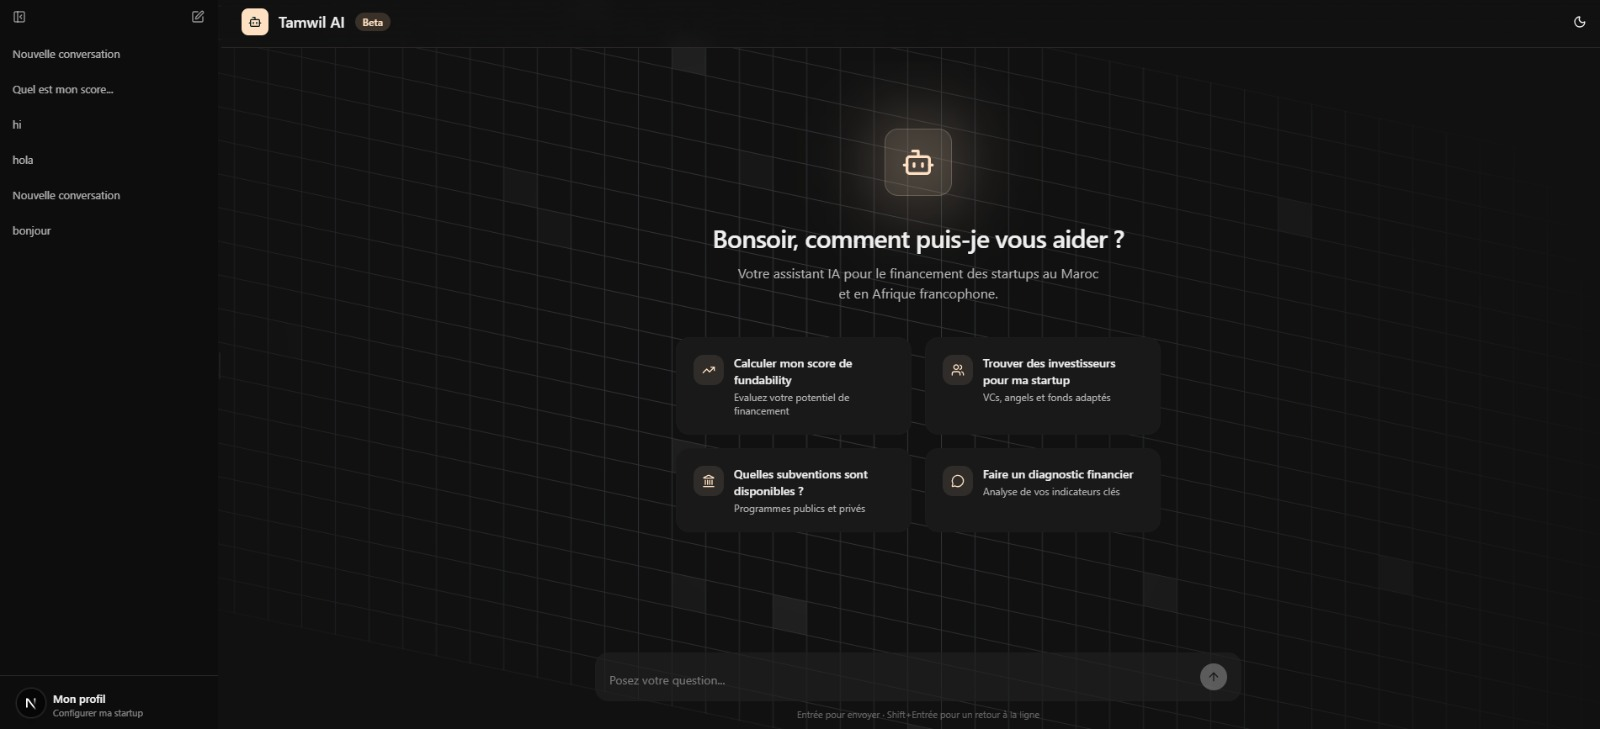
\includegraphics[width=\linewidth]{images/screenshots/ui_dark.jpeg}
  \captionsetup{labelformat=empty}
  \caption{\small (a) Mode sombre}
\end{minipage}\hfill
\begin{minipage}[b]{0.48\textwidth}
  \centering
  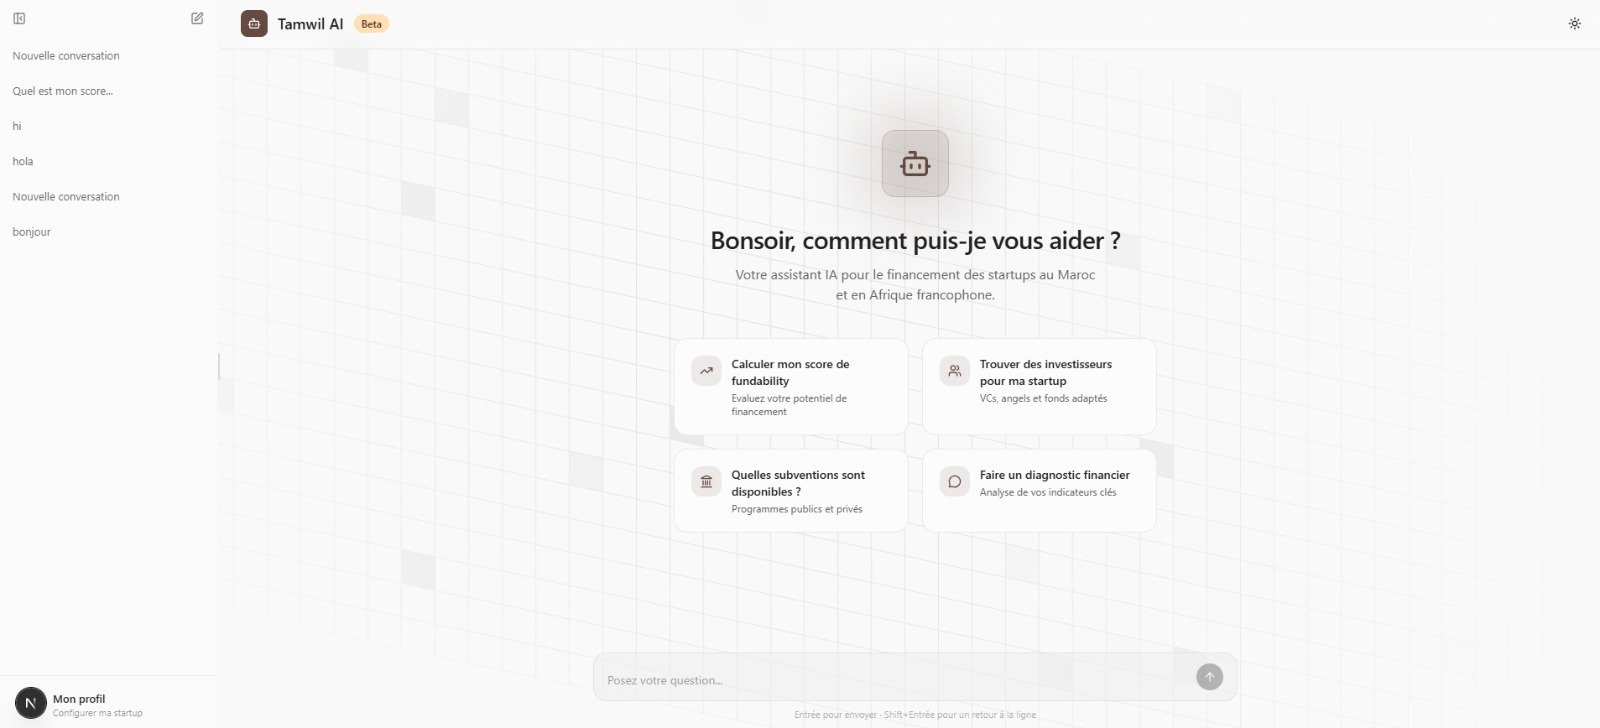
\includegraphics[width=\linewidth]{images/screenshots/ui_light.jpeg}
  \captionsetup{labelformat=empty}
  \caption{\small (b) Mode clair}
\end{minipage}
\caption{Interface d'accueil de Tamwil~AI en mode sombre et en mode clair. La barre latérale affiche l'historique des conversations~; la zone centrale présente un message de bienvenue et quatre cartes de suggestion (score de \textit{fundability}, recherche d'investisseurs, subventions, diagnostic financier).}
\label{fig:ui_themes}
\end{figure}

\subsection{Gestion d'état et consommation du flux SSE}

L'état global est géré dans \code{page.tsx} avec les \textit{hooks} React natifs~: \code{conversations} et \code{profile} sont persistés dans le \code{localStorage}. La consommation du flux \ac{SSE} se fait dans \code{lib/api.ts} via \code{ReadableStream} et \code{TextDecoder}, avec des \textit{callbacks} dédiés (\code{onSources}, \code{onToken}, \code{onReply}, \code{onDone}).

\section{Structure du projet}

Le dépôt est organisé comme suit~:

\begin{lstlisting}[language=bash, caption={Structure simplifiée du dépôt.}]
tamwil-ai/
|-- backend/
|   |-- app/
|   |   |-- config.py                 # Configuration centralisee
|   |   |-- main.py                   # Serveur FastAPI (3 endpoints)
|   |   |-- router.py                 # Routeur / detection d'intention
|   |   |-- source_urls.py            # Mapping fichiers -> URLs
|   |   |-- modules/
|   |   |   |-- scoring.py            # Scoring /100
|   |   |   |-- diagnostic.py         # Diagnostic financier
|   |   |   |-- matching_investors.py # Matching 0-4
|   |   |   |-- matching_grants.py    # Matching subventions
|   |   |   `-- rag_qa.py             # Q&A streaming
|   |   |-- rag/
|   |   |   |-- ingest.py
|   |   |   |-- embeddings.py
|   |   |   |-- vectorstore.py
|   |   |   `-- retriever.py
|   |   `-- utils/
|   |       `-- data_loader.py
|   `-- .env
|-- dataset/
|   |-- investors/investors.json       # 41 profils
|   |-- grants/grants.json             # 25 programmes
|   |-- metrics/metrics_reference.json # 18 KPIs
|   |-- faq/faq.json                   # 54 Q&A
|   |-- fundraising_guide/*.md         # 6 guides
|   `-- regulations/*.md               # 4 documents
|-- chroma_db/                         # Base vectorielle (9,4 MB)
|-- frontend/src/                      # Interface Next.js
|-- tests/                             # 6 fichiers pytest
`-- requirements.txt
\end{lstlisting}

\section{Règles de développement}

\begin{enumerate}
  \item \textbf{Langue}~: le code et les commentaires sont en anglais~; les \textit{prompts}, les réponses utilisateur et les données sont en français.
  \item \textbf{Pas d'hallucination}~: le \ac{LLM} ne répond qu'à partir du contexte \ac{RAG} ou des données structurées~; le \textit{system prompt} l'interdit explicitement de fabriquer des sources.
  \item \textbf{Modularité}~: chaque module est indépendant et testable séparément~; les fonctions publiques retournent des types de données simples (\textit{dict} Python).
  \item \textbf{Gestion d'erreurs}~: les données manquantes ou incomplètes sont gérées gracieusement (\textit{logging}, valeurs par défaut) plutôt que par des exceptions fatales.
  \item \textbf{ChromaDB persistant}~: la base vectorielle n'est pas reconstruite à chaque démarrage~; \code{build\_vectorstore()} est appelé à la demande.
  \item \textbf{Streaming}~: seul le Q\&A \ac{RAG} utilise le \textit{streaming}~; les autres intentions renvoient la réponse en un bloc pour garantir l'atomicité du formatage.
\end{enumerate}
